\documentclass[journal]{IEEEtran}

\usepackage{tikz}
\usetikzlibrary{shapes.geometric, arrows, positioning, calc}

\usepackage[T1]{fontenc}
\usepackage{amsmath,amsfonts}
\usepackage{newtxtext}
\usepackage{newtxmath}

\usepackage{algorithmic}

\usepackage{cite}
\usepackage{graphicx}
\usepackage{tabularx}
\usepackage{booktabs}

\usepackage[utf8]{inputenc}
% \usepackage[landscape]{geometry}

\usepackage[hidelinks]{hyperref}

\begin{document}

\title{Analysis of Anxiety Level Across Various Auditory Conditions}

\author{Andy Babcock \\
    \textit{Steve Sanghi College of Engineering, Northern Arizona University} \\
    Flagstaff, AZ, USA \\
    aab726@nau.edu
}

\maketitle

\section{Introduction}
This analysis will make little sense if reading after the previous assignments, as the majority of this wearable project has been re-done in the past two weeks. Cameron and I are using a NeuroSky Mindwave Mobile 2 to measure anxiety and cognitive load under various stress levels and auditory conditions. To achieve this, we adapted Peplau's definitions of anxiety levels~\ref{tab:peplau_anxiety_1952} into broader definitions that apply to general cognitive load. In our case, we defined Level 1 as a calm resting state, like meditating or reading. Level 2 was a cognitive load with a punishment for failure: taking a typing test where a mistake resets the string of words, or taking a Stroop test. The Stroop test traditionally shows one of four words, red, green, blue, or yellow, in one of those colors, and the participant must say the color of the word, not the word (i.e.: the word is red, and that text is green)~\cite{MacLeodColinM1991HaCo}. This test was adapted to instead press one of four buttons when a colored word appeared on-screen to remove the talking element. Level 3 would involve a task too difficult to properly do in the allotted time with a significant punishment for failure. However, Cameron and I are still deliberating between testing additional auditory conditions, like a loud room, podcast, or unfamiliar music, or testing the current conditions, white noise and familiar music, with a level 3 task.

The backbone of our EEG brainwave analysis is a recently developed EEG model, SingLEM~\cite{SukhbaatarJamiyan2025SSLE}. This general-purpose pre-trained model was trained on 357,000 hours of single-channel EEG data, and handles the large amount of noise inherent to single-channel EEG readings, like blinks and eye movement.

\begin{table}[htbp]
\centering
\caption{Peplau's Four Levels of Anxiety and their Effect on Perception and Behavior~\cite[pp. 126--133]{peplau1952interpersonal}.}
\label{tab:peplau_anxiety_1952}
\renewcommand{\arraystretch}{1.5} % Adds slight padding for readability
\begin{tabularx}{\linewidth}{@{} l >{\raggedright\arraybackslash}X @{}}
\toprule
\textbf{Anxiety Level} & \textbf{Perceptual Field \& Cognition} \\ 
\midrule
\textbf{1. Mild} & 
\textbf{Minimal narrowing.} Alertness is increased, allowing the individual to take more facets of a situation into account. Serves as a "functionally effective element" that mobilizes resources for problem-solving. \\ 

\textbf{2. Moderate} & 
\textbf{Narrowed awareness.} Forces are focused upon a smaller area of living. Employs "selective inattention" where peripheral aspects of experience are ignored to permit strict concentration on the immediate problem. \\ 

\textbf{3. Severe} & 
\textbf{Cripplingly narrowed.} The individual sees less and takes less into account. There is a gross inability to consider facts, evidence, or the broader situation. Alertness is significantly reduced. \\ 

\textbf{4. Panic} & 
\textbf{Disorganized.} The personality disorganizes rapidly. The individual cannot observe what is happening or collaborate in resolving the situation. \\ 
\bottomrule
\end{tabularx}
\vspace{1ex}
\end{table}

\section{Analysis}
SingLEM was finetuned using 30 minutes of each Level 1 and Level 2 data taken in silence, resulting in 82.9\% accuracy after 6 Epochs~\cite{jtof-dev_EE-499_2026}. The model was finetuned on 50 Epochs, using 80\% of the collected data to train and the remaining 20\% to validate that the model is not overfitting at the end of each Epoch. Then, after 50 Epochs, the generation with the highest accuracy and lowest loss between the training and validation is selected as the best-fit fine-tune. To get usable results, our data was filtered through multiple filters to eliminate external electrical noise, downsampled to match how SingLEM was trained, and the baseline calibrated through Z-Score normalization. The Z-Score normalization ensures that the model is 'centered' on our data, rather than comparing it to the baseline it found during pre-training. Lastly, the pre-trained SingLEM is unfrozen so it can learn during the fine-tune, but at a slow learning rate (\(1e^-5)\), while classification portion of the model is trained much faster (\(1e^-3)\). 

After fine-tuning SingLEM on Level 1 and 2 data taken in silence, the Level 2 Stroop test was repeated with white noise playing and with familiar music. The model we trained is a binary classifier, and only outputs a 0 or a 1. To get detailed information on how close to Level 1 or 2 the participant is over time, the Expected Value is calculated over time~\ref{eq:expected_level}. This methodology avoids the sometimes inaccurate outputs from only using a softmax.

\begin{equation}
    \label{eq:expected_level}
    E[L] = (P_1 \times V_1) + (P_2 \times V_2)
\end{equation}

Where:
\begin{itemize}
    \item $E[L]$ is the Expected Level (continuous cognitive load score).
    \item $P_1$ is the Softmax probability assigned to Class 1.
    \item $V_1$ is the numerical value assigned to Level 1 ($V_1 = 1.0$).
    \item $P_2$ is the Softmax probability assigned to Class 2.
    \item $V_2$ is the numerical value assigned to Level 2 ($V_2 = 2.0$).
\end{itemize}

Comparing the three auditory conditions shows an increase in total average correct answers and average keys pressed, with silence being the lowest and music the highest~\ref{tab:participant_andy_metrics_total}. However, the overall accuracy decreased during the music tests, with silence being the most accurate. It is possible that the increased anxiety level in the silent and white noise conditions cause enough second-guessing and slowdowns to prevent additional errors that music did not~\ref{fig:graph1}.

\begin{table}[htbp]
    \centering
    \caption{Aggregated Stroop test metrics for Andy. Data reflects total averages per run across different auditory conditions~\cite{jtof-dev_EE-499_2026}.}
    \label{tab:participant_andy_metrics_total}
    \resizebox{\linewidth}{!}{%
        \begin{tabular}{l c c c c c c}
            \toprule
            \textbf{Condition} & \textbf{Runs} & \textbf{Avg Keys} & \textbf{Avg Correct} & \textbf{Avg Errors} & \textbf{Keys/Sec} & \textbf{Accuracy (\%)} \\
            \midrule
            Silent     & 3 & 399.7 & 376.7 & 23.0 & 1.34 & 94.25 \\
            WhiteNoise & 2 & 432.5 & 403.0 & 29.5 & 1.45 & 93.18 \\
            Music      & 2 & 491.0 & 448.0 & 43.0 & 1.65 & 91.24 \\
            \bottomrule
        \end{tabular}%
    }
\end{table}

\section{Conclusion}
In order of conditions from silent, white noise, to music, overall number of keys pressed and correct answers increased. However, accuracy decreased as the input speed increased, with the music condition resulting in 3\$ worse accuracy than the silent condition.

This dataset and analysis serves well as an initial baseline for comparing anxiety levels across different auditory conditions. However, the dataset will certainly need some Level 3 data to better ground the results, more data across all collected categories, and likely more auditory contitions. While the model appears to fine-tune well, 30 minutes of data is likely close to the minimum amount of data needed to produce a functional fine-tune. Adding more data, and preferably doubling it to 60 minutes of each, would increase the quality of the fine-tune. Additionally, there are only two five-minute samples on taking the Stroop test under various conditions, making the dataset small enough that random variance could effect the overall result. Lastly, though there was an increase in overall output in the familiar music samples, that may have been from growing more comfortable with the test itself; interleaving various conditions during testing would likely fix this.

\begin{figure*}[p] % forces a dedicated page
    \begin{minipage}[c][0.48\textheight][c]{\linewidth}
        \centering
        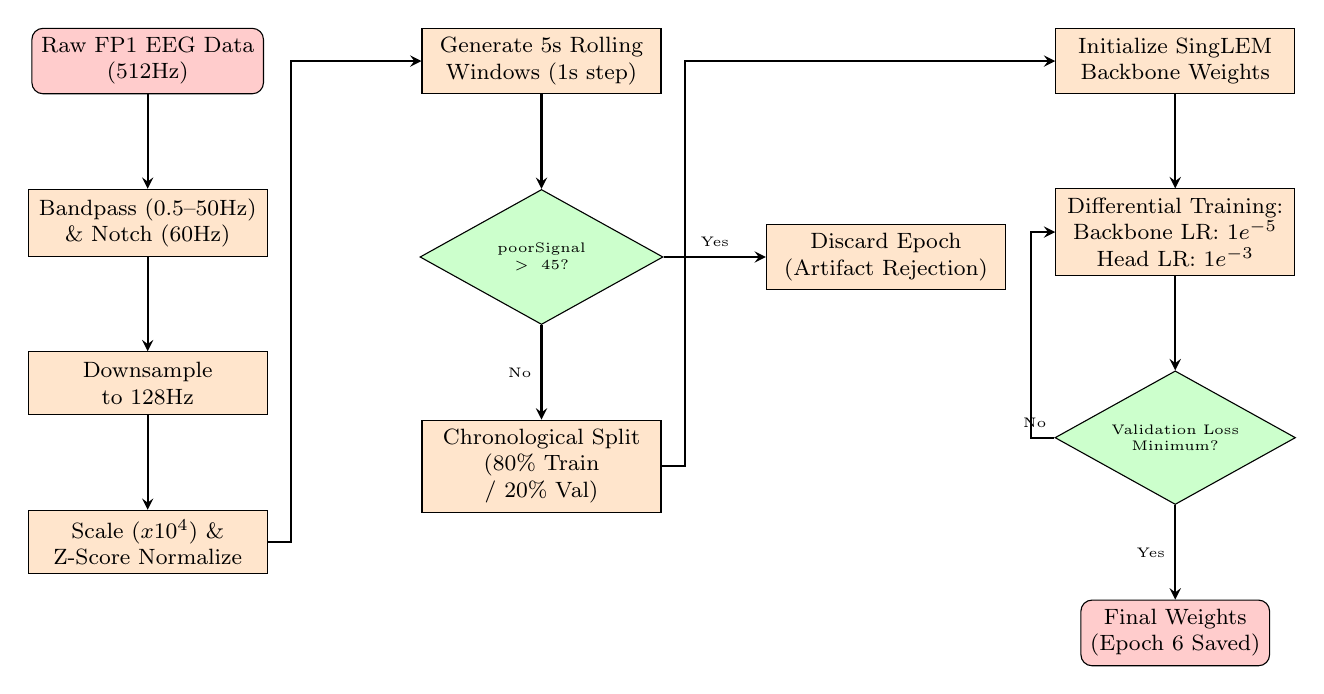
\begin{tikzpicture}[
            node distance=1.2cm and 0.8cm,
            auto,
            % styles
            startstop/.style={rectangle, rounded corners, minimum width=2.2cm, minimum height=0.8cm, text centered, draw=black, fill=red!20, font=\footnotesize, align=center},
            process/.style={rectangle, minimum width=2.5cm, minimum height=0.8cm, text centered, text width=2.8cm, draw=black, fill=orange!20, font=\footnotesize, align=center},
            decision/.style={diamond, aspect=1.8, minimum width=2cm, minimum height=0.8cm, text centered, text width=1.8cm, draw=black, fill=green!20, font=\tiny, align=center},
            arrow/.style={thick,->,>=stealth}
        ]

        % column 1: preprocessing
        \node (start) [startstop] {Raw FP1 EEG Data\\(512Hz)};
        \node (pro1)  [process, below=of start] {Bandpass (0.5--50Hz)\\ \& Notch (60Hz)};
        \node (pro2)  [process, below=of pro1] {Downsample\\to 128Hz};
        \node (pro3)  [process, below=of pro2] {Scale ($x 10^4$) \&\\ Z-Score Normalize};

        % column 2: windowing and rejection
        \node (pro4)  [process, right=of start, xshift=1.2cm] {Generate 5s Rolling\\ Windows (1s step)};
        \node (dec1)  [decision, below=of pro4] {poorSignal $> 45$?};
        \node (pro5)  [process, right=of dec1, xshift=0.5cm] {Discard Epoch\\(Artifact Rejection)};
        \node (pro6)  [process, below=of dec1] {Chronological Split\\(80\% Train / 20\% Val)};

        % column 3: training
        \node (pro7)  [process, right=of pro4, xshift=4.2cm] {Initialize SingLEM\\ Backbone Weights};
        \node (pro8)  [process, below=of pro7] {Differential Training:\\ Backbone LR: $1e^{-5}$\\ Head LR: $1e^{-3}$};
        \node (dec2)  [decision, below=of pro8] {Validation Loss\\ Minimum?};
        \node (stop)  [startstop, below=of dec2] {Final Weights\\ (Epoch 6 Saved)};

        % connections
        \draw [arrow] (start) -- (pro1);
        \draw [arrow] (pro1) -- (pro2);
        \draw [arrow] (pro2) -- (pro3);

        % transition col 1 to col 2
        \draw [arrow] (pro3.east) -- ++(0.3,0) |- (pro4.west);

        \draw [arrow] (pro4) -- (dec1);
        \draw [arrow] (dec1) -- node[anchor=south, font=\tiny] {Yes} (pro5);
        \draw [arrow] (dec1) -- node[anchor=east, font=\tiny] {No} (pro6);

        % transition col 2 to col 3
        \draw [arrow] (pro6.east) -- ++(0.3,0) |- (pro7.west);

        \draw [arrow] (pro7) -- (pro8);
        \draw [arrow] (pro8) -- (dec2);
        \draw [arrow] (dec2) -- node[anchor=east, font=\tiny] {Yes} (stop);

        % feedback loop for dec 2
        \draw [arrow] (dec2.west) -- node[anchor=south, font=\tiny, xshift=-0.1cm] {No} ++(-0.3,0) |- (pro8.west);

        \end{tikzpicture}
        \caption{System Architecture: EEG preprocessing, artifact rejection, and SingLEM fine-tuning with automated Early Stopping.}
        \label{fig:methodology_flow}
    \end{minipage}

    \vfill

    \begin{minipage}[c][0.48\textheight][c]{\linewidth}
        \centering
        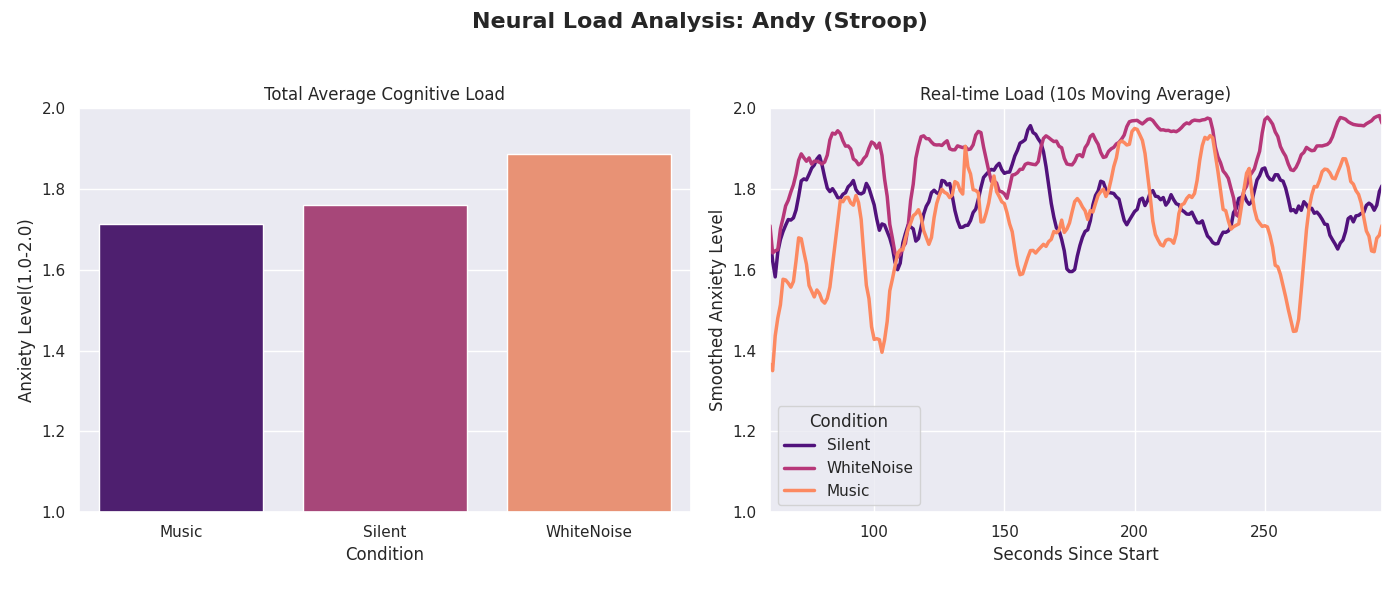
\includegraphics[width=\textwidth]{figures/neural_load_analysis.png}
        \caption{Overall and Real-Time Anxiety Level~\cite{jtof-dev_EE-499_2026}.}
        \label{fig:graph1}
    \end{minipage}
\end{figure*}

\bibliographystyle{IEEEtran}
\bibliography{references}

\end{document}
